\chapter{Competition for Authenticated Encryption: Security, Applicability and Robustness}
\label{toc/caesar}

In 2013, CAESAR was announced. It is a worldwide cryptographic competition, focused on finding new methods of authenticated encryption, that offer advantages against commonly used AES-GCM and will be suitable for widespread adoption. Submitted algorithms will be publicly evaluated by committee of researchers in fields of cryptography and cryptoanalysis.

This competition follows a long tradition of focused competitions in secret-key cryptography:

\begin{itemize}
  \item In 1997, United States National Institute of Standards and Technology (NIST) announced an open competition for a new symmetric cupher, Advanced Encryption Standard (AES). This competition attracted 15 submissions from 50 cryptographers around the world. In the end, Rijndael was chosen as AES.
  \item In 2004, European Network of Excellence in Cryptology (ECRYPT) announced the ECRYPT Stream Cipher Project (eSTREAM), a call for new stream ciphers suitable for widespread adoption. This call attracted 34 submissions from 100 cryptographers around the world. In the end, the eSTREAM committee selected a portfolio containing several stream ciphers.
  \item In 2007, NIST announced an open competition for a new hash standard to Secure Hash Algorithm family (SHA-3). This competition attracted 64 submissions from 200 cryptographers around the world. In the end, Keccak was chosen as SHA-3.
\end{itemize}

All past cryptographic competitions attracted many submissions from cryptographers around the world, and then even more security and performance evaluations from cryptanalysts. They are generally viewed as having provided a tremendous boost to the cryptographic research community's understanding of underlying concepts, and a tremendous increase in confidence in the security of some existing cryptosystems. Similar comments are expected to apply to CAESAR. \cite{crypto-competitions}


\section{Requirements}

\subsection{Functional requirements}

For the purpose of CAESAR competition, an \textit{authenticated cipher} is a pair of encrypt and decrypt functions, meeting the following specific requirements.

All inputs and outputs should be represented as opaque byte-strings (members of a set $\mathbb{Z}_{2^8}^*$), because they benefit from direct support of current computers to store and transmit them.

A cipher is permitted to be defined using objects other then byte-strings, nevertheless it must specify an unambiguous relationship between those objects and byte-strings (e.g. endianness of integers).

A cipher must specify a length of all fixed-length inputs. It is permitted to specify a maximum length of various-length inputs, but this limit must not be smaller than 65 kB and submissions are expected to include justification for any maximum length limits.

No other restrictions on their structure should be imposed, all inputs meeting the length restrictions must be accepted.

\subsubsection{Inputs and outputs}

\newcommand{\boldYes}[1]{%
  \ifthenelse{\equal{#1}{yes}}{\textbf{#1}}{#1}%
}

\begin{table}
  \centering
  \csvreader[
    after head=\begin{tabular}{lllll}\toprule\csvlinetotablerow\\\midrule,
    late after line=\\,
    late after last line=\\\bottomrule\end{tabular}
  ]
    {tables/caesar-inputs.csv}{}
    {\csvcoli & \boldYes{\csvcolii} & \boldYes{\csvcoliii} & \boldYes{\csvcoliv} & \boldYes{\csvcolv}}

  \caption{CAESAR inputs}
  \label{table/caesar-inputs}
\end{table}


A \textit{plaintext} is a variable-length input/output, a piece of confidential information a sender wants to transmit to a receiver, as introduced in \autoref{toc/encryption}.

A \textit{ciphertext} is a variable-length input/output counterpart of the plaintext, that can be transmitted over an insecure channel. it is usually longer then the plaintext, because it contains an \textit{authentication tag}. This length difference is permitted to be fixed constant, thus leaking the plaintext length via the ciphertext length. Designers are advised that minimizing ciphertext length is generally considered more valuable than hiding plaintext length.

A \textit{key} is a fixed-length input, which determines the output of both encrypt and decrypt functions. The key must be shared between both communicating parties prior to encrypted communication. Without a key or with a different one then used in the encrypt function, the decrypt function produces no useful result. This follows the Kerckhoffs' principle as introduced in \autoref{toc/kerckhoffs-principle}.

An \textit{associated data} is a variable-length input, a piece of information known by both communicating parties, which does not need to meet confidentiality requirement. However, its origin still needs to be verified by the receiving party. It can be for example some message metadata, such as version of used protocol.

A \textit{nonce} (number used once) is a fixed-length input. It is a public value, which which is usually used as IV for the enclosed cipher. Such IVs should be unique for each encryption run, so it makes all ciphertexts undistinguishable even if the same key, message and associated data is used.

However, CAESAR call for submissions requests an unusual authenticated encryption interface. The user, who wants to encrypt, instead of providing the usual \textit{four} arguments (the key, nonce, associated data, and message) for authenticated encryption, he needs to provide \textit{five} arguments. The nonce has been transformed into a \textit{public message number} and \textit{secret message number}. \cite{cryptoeprint:2013:242}

A \textit{public message number} is a fixed-length input. It is a public value with the same requirements as the nonce in the original definition of authenticated encryption.

A \textit{secret message number} is a fixed-length input. It is a secret value, recoverable from the ciphertext, however it is not a part of the plaintext. Allowing both a secret message number and a public message number creates possibilities of different levels of their security requirements.

All inputs must meet various security purposes, as indicated by \autoref{table/caesar-inputs}.


\subsection{Software requirements}
\label{toc/caesar-api}

Each first-round submission must contain a portable reference software implementation to support public understanding of the cipher, cryptanalysis, verification of subsequent implementations, etc. The implementation must cover all recommended parameter sets, and must compute exactly the function specified in the submission. The reference implementation is expected to be optimized for clarity, not for performance. \cite{crypto-competitions}

The submission must export the following constants:

\begin{itemize}
  \item \texttt{CRYPTO\_KEYBYTES} -- the fixed length of key
  \item \texttt{CRYPTO\_NSECBYTES} -- the fixed length of secret message number (0 if not supported)
  \item \texttt{CRYPTO\_NPUBBYTES} -- the fixed length of public message number (0 if not supported)
  \item \texttt{CRYPTO\_ABYTES} -- the maximum (usually fixed) length difference between plaintext and ciphertext
\end{itemize}

\inputminted{c}{code/caesar/constants.c}

The submission must export the following \texttt{crypto\_aead\_encrypt} and \texttt{crypto\_aead\_decrypt} functions, which perform the encrypt and decrypt operation respectively.

\inputminted{c}{code/caesar/encrypt.c}
\inputminted{c}{code/caesar/decrypt.c}

The output of functions must be determined entirely by the inputs in their arguments and must not be affected by any randomness or other hidden inputs.

The functions should perform the operation in constant time with regard to any input data (even invalid data) to prevent timing side-channel attacks.

The decrypt function must return -1 if the ciphertext is not valid, i.e. if the ciphertext does not equal the encryption of any (plaintext, secret message number) pair with this associated data, public message number, and secret key. The functions may return other negative numbers to indicate other failures, for example memory-allocation failures. \cite{crypto-competitions}


\subsection{Hardware requirements}

Each submission selected for the second round will also be required to include a reference hardware design (i.e., a reference implementation in the VHDL or Verilog languages). Details of the hardware API have not yet been specified. \cite{crypto-competitions}

\section{Submissions}

The competition was announced on 2013-01-15 at the Early Symmetric Crypto workshop in Mondorf-les-Bains, also announced online\footnote{\url{https://groups.google.com/d/forum/crypto-competitions}}. First-round submission papers must have been received till 2014-03-15, reference software implementations must have been received till 2014-04-15.

After passing the first-round deadline, all submissions were published. All submission papers can be downloaded on CAESAR homepage\footnote{\url{http://competitions.cr.yp.to/caesar-submissions.html}}. Submission source codes are bundled together with SUPERCOP benchmark application\footnote{\url{http://bench.cr.yp.to/supercop.html}}. There is a website with SUPERCOP speed benchmark results\footnote{\url{http://www1.spms.ntu.edu.sg/~syllab/speed/}}.

Also there was Directions in Authenticated Ciphers (DIAC) 2014 conference, where a lot of sumbission authors presented their candidates. Talk slides are available for download on the DIAC website\footnote{\url{http://2014.diac.cr.yp.to/index.html}}.

There were submitted 57 candidates for the CAESAR competition. A good insight into their classification is provided by Authenticated Encryption Zoo\footnote{\url{https://aezoo.compute.dtu.dk/}}. At the time of writing this thesis, 9 candidates (AES-COBRA, Calico, CBEAM, FASER, HKC, Marble, McMambo, PAES and PANDA) are considered broken and were withdrawn from the competition, because a cryptanalysis was published that broke the security claim made by the designers. \cite{cryptoeprint:2014:792} There are 48 candidates remaining. It is expected that the about a half of them will advance to the second round.

Announcement of second-round candidates was initially scheduled for 2015-01-15. However it is a hard task to do a proper security review, analysis and comparison of all submissions. Currently in the time of writing this thesis, the second-round candidates announcement is being postponed every month.


\subsection{Overall construction}

\begin{figure}
  \centering
  \begin{minipage}{0.8\textwidth}
    \raggedleft
    \begin{tikzpicture}
      \node (table) [matrix,row sep=1.5*\nodeheight,column sep=\nodeheight] {
        \node (plaintext1) [smallrect] {$m_1$}; & \node (plaintext2) [smallrect] {$m_2$}; & \node (plaintext3) [smallrect] {$m_3$}; \\
        \node (encryption1) [circle] {$E_K$}; & \node (encryption2) [circle] {$E_K$}; & \node (encryption3) [circle] {$E_K$}; \\
        \node (ciphertext1) [smallrect] {$c_1$}; & \node (ciphertext2) [smallrect] {$c_2$}; & \node (ciphertext3) [smallrect] {$c_3$}; \\
      };
      \path [line] (plaintext1) -- (encryption1);
      \path [line] (plaintext2) -- (encryption2);
      \path [line] (plaintext3) -- (encryption3);
      \path [line] (encryption1) -- (ciphertext1);
      \path [line] (encryption2) -- (ciphertext2);
      \path [line] (encryption3) -- (ciphertext3);

      \node (table2) [matrix,right=1 of table,row sep=\nodeheight,column sep=\nodeheight] {
        \node (plaintext) {
\includegraphics[scale=0.25]{images/tux.jpg}}; \\
        \node (ciphertext) {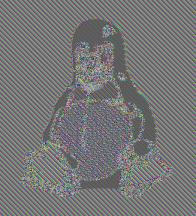
\includegraphics[scale=0.25]{images/tux-ecb.jpg}}; \\
      };
      \path [line] (plaintext) -- (ciphertext);
    \end{tikzpicture}
    \subcaption{ECB block mode}
  \end{minipage}
  \begin{minipage}{0.8\textwidth}
    \raggedleft
    \begin{tikzpicture}
      \node (table) [matrix,row sep=1.5*\nodeheight,column sep=\nodeheight] {
        \node (iv) [smallrect] {$IV$}; & \node (plaintext1) [smallrect] {$m_1$}; & \node (plaintext2) [smallrect] {$m_2$}; & \node (plaintext3) [smallrect] {$m_3$}; \\[-0.75*\nodeheight]
        & \node (plaintext1_after) [inner sep=0] {\Large $\oplus$}; & \node (plaintext2_after) [inner sep=0] {\Large $\oplus$}; & \node (plaintext3_after) [inner sep=0] {\Large $\oplus$}; \\[-0.75*\nodeheight]
        & \node (encryption1) [circle] {$E_K$}; & \node (encryption2) [circle] {$E_K$}; & \node (encryption3) [circle] {$E_K$}; \\[-0.75*\nodeheight]
        & \coordinate (ciphertext1_before) [inner sep=0]; & \coordinate (ciphertext2_before) [inner sep=0]; & \coordinate (ciphertext3_before) [inner sep=0]; \\[-0.75*\nodeheight]
        & \node (ciphertext1) [smallrect] {$c_1$}; & \node (ciphertext2) [smallrect] {$c_2$}; & \node (ciphertext3) [smallrect] {$c_3$}; \\
      };
      \path [line] (plaintext1) -- (plaintext1_after);
      \path [line] (plaintext2) -- (plaintext2_after);
      \path [line] (plaintext3) -- (plaintext3_after);
      \path [line] (plaintext1_after) -- (encryption1);
      \path [line] (plaintext2_after) -- (encryption2);
      \path [line] (plaintext3_after) -- (encryption3);
      \path [line] (encryption1) -- (ciphertext1);
      \path [line] (encryption2) -- (ciphertext2);
      \path [line] (encryption3) -- (ciphertext3);
      \path [line] (iv) |- (plaintext1_after);
      \path [line] (ciphertext1_before) -| ($(encryption1) !.5! (encryption2)$) |- (plaintext2_after);
      \path [line] (ciphertext2_before) -| ($(encryption2) !.5! (encryption3)$) |- (plaintext3_after);

      \node (table2) [matrix,right=1 of table,row sep=\nodeheight,column sep=\nodeheight] {
        \node (plaintext) {
\includegraphics[scale=0.25]{images/tux.jpg}}; \\
        \node (ciphertext) {
\includegraphics[scale=0.25]{images/tux-cbc.jpg}}; \\
      };
      \path [line] (plaintext) -- (ciphertext);
    \end{tikzpicture}
    \subcaption{CBC block mode}
    \bigskip
  \end{minipage}

  \begin{footnotesize}
    The ECB mode is the most basic block mode, which does not perform any block feedback. Note that the plaintext structure is still observable in the ciphertext.
  \end{footnotesize}

  \caption{Basic block modes}
  \label{figure/block-modes}
\end{figure}

\begin{figure}
  \begin{minipage}{\textwidth}
    \centering
    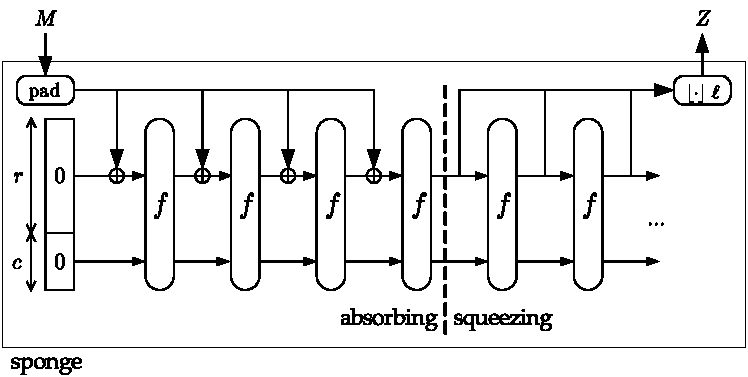
\includegraphics[scale=0.8]{images/sponge.pdf}
    \subcaption{The sponge construction}
  \end{minipage}
  \begin{minipage}{\textwidth}
    \centering
    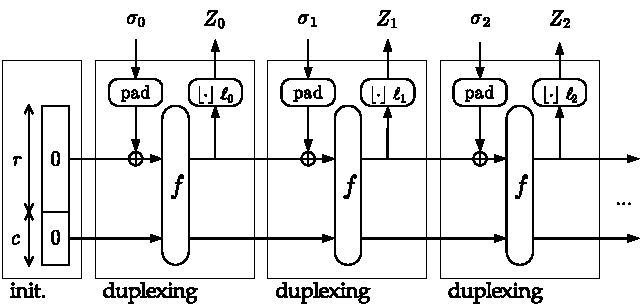
\includegraphics[scale=0.8]{images/duplex.pdf}
    \subcaption{The duplex construction}
  \end{minipage}

  \caption{Sponge functions}
  \label{figure/sponge-functions}
\end{figure}


Most of first-round candidates can be classified according to their construction design approaches. \cite{cryptoeprint:2014:792}

\begin{description}
  \item[Block Cipher] A block cipher is a bijective keyed permutation $E: \{0, 1\}^k \times \{0, 1\}^n \rightarrow \{0, 1\}^n, E(K, P) = C$, parametrized by a secret key $K$ of length $k$, and that takes as input a plaintext message $p$ of length $n$, and outputs a ciphertext message $c$ of length $n$. The permutation is used for encryption, an inverted permutation is used for decryption. A block mode is usually accompanied with a block mode.
  \begin{description}
    \item[Block Mode] A block mode (also called mode of operation) is used by block ciphers for secure transformation of data larger than a single block. See \autoref{figure/block-modes} for basic block modes. Some submissions defines only a new block mode and relies on existing block cipher (e.g. AES). \cite{cryptoeprint:2014:186} \\
    Example candidates: COBRA, JAMBU, POET
  \end{description}
  \item[Stream Cipher] A stream cipher is a pseudo-random generator, that takes a fixed-length secret key and generates a keystream of variable length. The keystream is combined with the plaintext message to produce ciphertext message and vice versa. The combining operation is usually XOR. \\
  Example candidates: ACORN, Morus
  \item[Key-Less Permutation] A key-less permutation is a bijective permutation on fixed-length strings. The key is sent to the permutation alongside the input, thus changing the internal state, effectivelly encrypting the output and producing the MAC tag.
  \begin{description}
    \item[Sponge Function] A sponge function is a generalization of both hash functions, which have a fixed output length, and stream ciphers, which have a fixed input length. It is a simple iterated construction for building a function with variable-length input and arbitrary-length output based on a fixed-length permutation. The inner permutation operates on a finite state of $b = r + c$ bits. The value $r$ is called the bitrate and the value $c$ the capacity. The sponge construction operates on the state by iteratively applying the inner permutation to it, interleaved with the entry of input or the retrieval of output, chunked by bitrate size. Literally, the sponge is said to \textit{absorb} its inputs block by block first before it processes and \textit{squeezes} it out afterwards. \cite{sponge-functions} \\
    A duplex sponge construction is closely related to the sponges. However unlike sponges, which are stateless between calls, the duplex construction allows alternation of input and output blocks at the same rate, like a full-duplex communication. Which means that it requires only one call of the inner permutation per input block. \cite{duplex-functions} See \autoref{figure/sponge-functions} for comparison. \\
    Example candidates: Ascon, ICEPOLE, Keyak, NORX, STRIBOB
  \end{description}
\end{description}


\subsection{Underlying primitive}

Under the overall construction usually hides a cryptographic primitive (e.g. inner permutation in sponge construction), which does the heavy lifting.

\begin{description}
  \item[AES] A lot of submissions use AES cipher or some of its parts (e.g. its round function), because during the years, AES have been enormously analysed in detail, and it is still believed to be secure. Moreover, starting with Intel's Westmere microarchitecture in 2011, current processors provide AES native instructions (AES-NI), that allow hardware-accelerated fast constant-time encryption and decryption.
  \item[Other named primitive] e.g. SHA2, Keccak, ChaCha, Streebog, etc.
  \item[Generic primitive type] e.g. Linear Feedback Shift Register (LSFR), Addition Rotation XOR (ARX), Logic Rotation XOR (LRX), Substition Permutation Network (SPN), etc.
\end{description}


\subsection{Functional characteristics, selection criteria}

The selection of second-round candidates will focus not only on general security of the scheme, but no less on important functional characteristics, which are good to have.

\begin{description}
  \item[High Security] The schema should be secure against all known kinds of cryptanalysis.
  \item[High Speed] The schema should be fast enough to compete with existing ciphers. However it is arguable whether the speed can be achieved by hardware acceleration such as by AES-NI or SIMD (SSE2, AVX2) instruction sets, because it does not need to be available on all platforms.
  \item[Simplicity] Clean design principles simplify cryptanalysis and allow a straightforward implementation in software and hardware.
  \item[Minimum Overhead] The ciphertext will be always larger than the plaintext, because it needs to include the MAC tag. However, this length difference should be minimal.
  \item[Side-Channel Robustness] The schema should resist against timing side-channel attacks, e.g. by avoiding data-dependant table look-ups (S-Boxes) or integer arithmetrics.
  \item[Parallelizable] An operation is parallelizable if the processing an input block does not depend on the output of processing any other block. Parallelizable encryption and decryption is considered separately.
  \item[Online] A cipher is called online if the processing an input block depends only on the output of processing of previous blocks and only constant size-state is used from the processing of one block to the next. It effectivelly means that the MAC tag must be computed during encryption, thus online schemes can be called one-pass. Such schemes can be faster in general. Schemes that are not online are called offline or two-pass.
  \item[Inverse-Free] A scheme is called inverse-free if it does not require either its underlying primitive inverse operation, e.g. as does require the block cipher's decryption function. Such scheme can save precious memory and circuit area resources.
  \item[Nonce Misuse-Resistance] States the robustness of the scheme when nonces are repeated. This property avoids maintaining a nonce generator.
\end{description}

\section{Selection}

Because the announcement of second-round candidates is in the time of writing this thesis still being postponed, I couldn't choose a well-rated candidate, which I would implement into OpenSSL. So I decided to implement a generic cipher using the CAESAR API (see \autoref{toc/caesar-api}).

As a reference cipher for my implementation part I chose NORX. It is not important which particular cipher I used, because the cipher can be easily switched for a different cipher complying with the CAESAR API, as soon as the the second-round candidate or final announcement will be made.

